\documentclass[12pt]{article}
\usepackage[utf8]{inputenc}
\usepackage{fontspec}
\setmainfont{Times New Roman}
\usepackage{tikz}
\usepackage{tikz-qtree}
\usepackage{tree-dvips}
\usepackage{amsmath}
\usepackage{indentfirst}
\usepackage{graphicx}
\usepackage{subfigure}
\usepackage{float}
\setlength{\parindent}{2em}
\usepackage{booktabs}
\usepackage{multirow}
\usepackage{listings}
\usepackage{geometry}
\usepackage{comment}
\usepackage{fancyhdr}
\usepackage{ctex}
\setlength{\headheight}{15pt}
\usepackage{algorithm}
\usepackage{algorithmic}
\pagestyle{fancy}
\fancyhf{}
\usepackage{mathrsfs}
\usepackage{amsfonts,amssymb}
\usepackage{pdfpages}
\usepackage{bm}
\definecolor{commentgreen}{rgb}{0.0 0.390625 0.0}
\makeatletter
\newenvironment{breakablealgorithm}
{% \begin{breakablealgorithm}
	\begin{center}
		\refstepcounter{algorithm}% New algorithm
		\hrule height.8pt depth0pt \kern2pt% \@fs@pre for \@fs@ruled
		\renewcommand{\caption}[2][\relax]{% Make a new \caption
			{\raggedright\textbf{\ALG@name~\thealgorithm} ##2\par}%
			\ifx\relax##1\relax % #1 is \relax
			\addcontentsline{loa}{algorithm}{\protect\numberline{\thealgorithm}##2}%
			\else % #1 is not \relax
			\addcontentsline{loa}{algorithm}{\protect\numberline{\thealgorithm}##1}%
			\fi
			\kern2pt\hrule\kern2pt
		}
	}{% \end{breakablealgorithm}
		\kern2pt\hrule\relax% \@fs@post for \@fs@ruled
	\end{center}
}
\makeatother

\lstset{
    basicstyle          =   \sffamily,          % 基本代码风格
    keywordstyle        =   \bfseries,          % 关键字风格
    commentstyle        =   \rmfamily\itshape,  % 注释的风格,斜体
    stringstyle         =   \ttfamily,  % 字符串风格
    flexiblecolumns,                % 别问为什么,加上这个
    numbers             =   left,   % 行号的位置在左边
    showspaces          =   false,  % 是否显示空格,显示了有点乱,所以不现实了
    numberstyle         =   \zihao{-5}\ttfamily,    % 行号的样式,小五号,tt等宽字体
    showstringspaces    =   false,
    captionpos          =   t,      % 这段代码的名字所呈现的位置,t指的是top上面
    frame               =   lrtb,   % 显示边框
}

\lstdefinestyle{Python}{
    language        =   Python, % 语言选Python
    basicstyle      =   \zihao{-5}\ttfamily,
    numberstyle     =   \zihao{-5}\ttfamily,
    keywordstyle    =   \color{blue},
    keywordstyle    =   [2] \color{teal},
    stringstyle     =   \color{orange},
    commentstyle    =   \color{commentgreen}\ttfamily,
    breaklines      =   true,   % 自动换行,建议不要写太长的行
    columns         =   fixed,  % 如果不加这一句,字间距就不固定,很丑,必须加
    basewidth       =   0.5em,
}
\lhead{Machine Learning}
\rhead{Created by He Entong}
\geometry{a4paper,scale=0.78}
\renewcommand{\figurename}{Fig.}
\newcommand{\bdot}{~\bm{\cdot}~}
\newcommand{\la}{\langle}
\newcommand{\ra}{\rangle}
\newcommand{\new}{\text{new}}
\newcommand{\old}{\text{old}}

\begin{document}
\section{K-Nearest Neightbour Algorithm}
\subsection{Basic Method}
The K-Nearest Neightbour Algorithm is an intuitive algorithm. Given an unknown sample, we compute its \textbf{Minkowski distance}
\begin{equation}
    \bm{d}(\bm{v_i}, \bm{v_j}) = \left( \sum_{k=1}^n (v_i^{(k)} - v_j^{(k)})^p\right)^{\frac{1}{p}}
\end{equation}
to elements in our training set, and use the average features of the K nearest elements picked out to predict the unknown one.
\subsection{Implementation}
\begin{algorithm}
    \caption{K-NN Algorithm ($S,~Vec$)}
    \label{K-NN}
    \begin{algorithmic}
        \REQUIRE{training set: $S$, sample vector $Vec = \{v_1, v_2, \dots, v_n\}$, hashmap $H$}
        \FOR{$s_i \in S$}
        \STATE{$d_i$ $\gets$ $\sqrt{\sum_{j=1}^n ((s_{i})_j - v_j)^2}$ (Using Euclidean distance)}
        \STATE{$H[s_i]$ = $d_i$}
        \ENDFOR
        \STATE{\textbf{sort} $H$ with key}
        \STATE{$array \gets$ $s_i|H[s_i]$ are K nearest}
        \STATE{$Vec.label$ = $\sum_{s_i \in array} \epsilon_i \cdot s_i.label$, $\epsilon_i = H[s_i] / \sum_{s_j \in array} H[s_j]$}
    \end{algorithmic}
\end{algorithm}
\subsection{Performance Analysis}
Assume that $\bm{x}$ is our testing vector, and the nearest training vector is $\bm{z}$. Then the generalizetion error is
\begin{equation}
    P_{\text{err}} = 1 - \sum_{c \in \mathcal{Y}}P(c|\bm{x})P(c|\bm{z})
\end{equation}
where $\mathcal{Y}$ is the label set. Then assume that the training set is dense enough, such that $\forall~\bm{x},~\exists~\delta,~\bm{z} \in \bm{x} + \delta$. The condition gives
\begin{equation}
    \begin{aligned}
    P_{\text{err}} &= 1 - \sum_{c \in \mathcal{Y}}P(c|\bm{x})P(c|\bm{z})\\ &\approx 1 - \sum_{c \in \mathcal{Y}}P^2(c|\bm{x}) \\
    &= 1 - \left(  \arg \max_{c \in \mathcal{Y}} P(c|x) \right)^2 \\
    &= \left( 1 -  \arg \max_{c \in \mathcal{Y}} P(c|x) \right) \left( 1 + \arg \max_{c \in \mathcal{Y}} P(c|x) \right) \leq 2 -  2 \arg \max_{c \in \mathcal{Y}} P(c|x)
    \end{aligned}
\end{equation}
This manifests that the error rate of K-NN will not exceed the double of the one of the Bayes optimal classifier.
\subsection{Code (with Python)}
\lstinputlisting[
    style       =   Python,
    caption     =   {\bf K-NN.py},
    label       =   {K-NN.py}
]{Numpy Files/K_NN.py}
\section{Decision Tree}
\subsection{Basic Model}
We tend to enable machines to do decision-making like humans.
The data structure we use is the decision tree, where each internal node corresponds to a characteristic testing $a_i$, and each leaf node denotes a final decision $y_i$. The core manipulation is to build up optimal classification at each node. Every top-down process on analyzing a sample corresponds to a testing sequence.
\begin{center}
\Tree [.{anterior feature}
        {feature 1} {$\cdots$}
        [.{feature n} {posterior-feature 1} {$\cdots$} [.{posterior-feature n} [.{$\cdots$} decision ] ] ] ]
\end{center}
\subsection{Partition Scenario}
\subsubsection*{Shannon Entropy}
For a decision set $D$, the \textbf{information size} $H_0(D)$ which denotes the number of bits needed to encode elements in $D$ is $H_0(D) = \log_{2}\lvert D\rvert$. Let $\bm{D} = (D, p)$ be a discrete probability space, where $D = \{D_1, D_2, \dots, D_n\}$ is a finite set, with $D_i$ corresponds to probability $p_i$ under definite discrete characteristic. Then the \textbf{Shannon entropy} of $\bm{D}$ is
\begin{equation}
    \text{Ent}(D) = -\sum_{i=1}^np_i\log_{2}p_i
\end{equation}
Since $-\log_{2}x$ is convex, we give an upper-bound for the entropy where
\begin{equation}
    -\log_{2}(\sum_{i=1}^n\frac{1}{p_i} p_i) \leq \sum_{i=1}^n p_{i}(-\log_{2}\frac{1}{p_i}) = -\text{Ent}(D)  \longrightarrow \text{Ent}(D) \leq \log_{2}n
\end{equation}
\subsubsection*{Information Gain}
Given a partition criterion $a = \{a^1, a^2, \dots, a^v\}$ where $a^i \in a$ is the possible value. For sample set $D$, we split it into subsets $D^1, D^2, \dots, D^v$ where $D^i$ is the subset determined by criterion $a^i$.
\begin{center}
\Tree [.$D$ $D^1$ $D^2$ $\cdots$ $D^v$ ]
\end{center}
Then the \textbf{information gain} we obtain from this partition is
\begin{equation}
    \text{Gain}(D, a) = \text{Ent}(D) - \sum_{i=1}^v \frac{\lvert D^i \rvert}{\lvert D \rvert} \text{Ent}(D^i)
\end{equation}
In ID3 Algorithm, the \textbf{optimal class partition} $a_{*}$ for $A$ with sample $D$ is defined as
\begin{equation}
    a_{*} = \arg \max_{a \in A} \text{Gain}(D, a)
\end{equation}
while for C4.5 Algorithm, the optimal one is defined as
\begin{equation}
    a_{*} = \arg \max_{a \in A} \text{GainRatio}(D,a),~~~\text{GainRatio}(D,a) = \text{Gain}(D,a) / \text{Ent}(D)
\end{equation}
\subsection{Implementation}
Assume that training sample set $D = \{(\bm{x_1}, y_1), (\bm{x_2}, y_2), \dots, (\bm{x_n}, y_n)\}$, where $\bm{x_i}$ is the class characteristics, and $y_i$ is the decision, eventually treated as leaftnode. Possible partition criterion for $D$ is $A = \{a_1, a_2, \dots, a_d\}$, where $a_i$ denotes a possible partition.
\begin{breakablealgorithm}
    \caption{treeGenerate($D$, $A$)}
    \label{treeGenerate}
    \begin{algorithmic}
        \REQUIRE{Training set $D$, Partition criterion set $A$}
        \STATE{\textbf{initialize} $node$}
        \IF{$\forall D_i D_j \in D, i \neq j,~D_i = D_j$}
        \STATE{$node = leafnode,~node \gets D.y$}
        \RETURN
        \ENDIF
        \IF{$A = \emptyset$ \OR $\forall a_i, a_j \in A, i \neq j,~\text{Gain}(D, a_i) = \text{Gain}(D, a_j)$}
        \STATE{$node = leafnode,~node \gets \arg \max_{y} (\lvert N \rvert,~N = \{y|(\bm{x}, y) \in D\})$}
        \ENDIF
        \STATE{$a_{*} \gets$ $\arg \max_{a \in A} \text{Gain}(D, a)$}
        \FOR{$a_{*}^v \in a_{*}$}
        \STATE{\textbf{initialize} $node.branch^v$, $D_v$ be the subset split with $a_{*}^v$}
        \IF{$D_v = \emptyset$}
        \STATE{$node.branch^v = leafnode$,~$node.branch^v \gets \arg \max_{y} (\lvert N \rvert,~N = \{y|(\bm{x}, y) \in D_v\})$ }
        \ELSE
        \STATE{{$node.branch^v$ = treeGenerate($D_v$, $A - \{a_{*}\})$}}
        \ENDIF
        \ENDFOR
    \end{algorithmic}
\end{breakablealgorithm}
\subsection{Code}
\lstinputlisting[
    style   =   Python,
    caption =   {\bf decisionTree.py},
    label   =   {decisionTree}
]{Numpy Files/decisionTree.py}
\section{Naive Bayes Algorithm}
\subsection{Principle and Method}
Given that the input vector $X \subseteq \mathbb{R}^n$, where $X = \begin{bmatrix} X^{(1)} & X^{(2)} & \cdots & X^{(n)} \end{bmatrix}^T$, and the relevant output class label set $Y \in \{c_1, c_2, \dots, c_K\}$. The joint distribution $P(X,Y)$ generates the data outcome
\begin{equation}
    T=\{(x_1, y_1),(x_2,y_2),\dots,(x_N,y_N)\}
\end{equation}
Applying Bayes rule we construct the algorithm for determining the label for an arbitrary new input.
\par
Assume that the input vector is $x = \begin{bmatrix}
x^{(1)} & x^{(2)} & \cdots & x^{(n)} \end{bmatrix}$, the probable label set is $\bm{c} = \{c_1, c_2, \dots, c_K\}$, then for $c_i \in \bm{c}$
\begin{equation}
    P(X = x|Y = c_i) = P\left( X^{(1)} = x^{(1)}, X^{(2)} = x^{(2)}, \dots, X^{(n)} = x^{(n)}| Y = c_i\right)
\end{equation}
Assume that the variables in $X$ are mutually independent, then the posteriori distribution is
\begin{equation}
    P(Y = c_i|X = x) = \frac{P(X = x|Y = c_i)P(Y=c_i)}{\sum_i^k P(X=x|Y = c_i)P(Y=c_i)} = \frac{\prod_{j}P(X^{(j)} = x^{(j)}|Y = c_i)P(Y=c_i)}{\sum_i \prod_{j}P(X^{(j)} = x^{(j)}|Y = c_i)P(Y=c_i)} \notag
\end{equation}
The optimal choice for $c_i$ is
\begin{equation}
\begin{aligned}
    y = f(x) = \arg \max_{c_i} P(Y = c_i|X = x) &= \arg \max_{c_i} \frac{ \prod_{j}P(X^{(j)} = x^{(j)}|Y = c_i)P(Y=c_i)}{\sum_i \prod_{j}P(X^{(j)} = x^{(j)}|Y = c_i)P(Y=c_i)} \\
    &= \arg \max_{c_i} \prod_{j}P(X^{(j)} = x^{(j)}|Y = c_i)P(Y=c_i)
\end{aligned}
\end{equation}
Assume that $x^{(j)} \in \bm{a_j} = \{a_{j,1}, a_{j,2}, \dots, a_{j,S_j}\}$, where $\bm{a_j}$ is the probable value set, then the apriori probability is
\begin{gather}
    P(Y = c_i) = \frac{\sum_{k=1}^N I(y_k = c_i)}{N} \notag \\
    P\left(X^{(j)} = a_{j,l}|Y = c_i \right) = \frac{\sum_{k=1}^N I(x_k^{(j)} = a_{j,l}, y_k = c_i)}{\sum_{k=1}^N I(y_k = c_i)} ~~~1 \leq l \leq S_{j},~1\leq j \leq n,~1 \leq i \leq K\notag
\end{gather}
\subsection{Laplace Smoothing}
When calculating the conditional probability, some special cases might annihilate the indicator random variable, where
\begin{equation}
    I(x_k^{(j)} = a_{j,l},y_k = c_i) = 0
\end{equation}
Then we use a coefficient  $\lambda$ to prevent. Redefine the probabilities as
\begin{gather}
    P(Y = c_i) = \frac{\sum_{k=1}^N I(y_k = c_i) + \lambda}{N + K \lambda} \notag \\
    P\left(X^{(j)} = a_{j,l}|Y = c_i \right) = \frac{\sum_{k=1}^N I(x_k^{(j)} = a_{j,l}, y_k = c_i) + \lambda}{\sum_{k=1}^N I(y_k = c_i) + S_j \lambda}
\end{gather}
When $\lambda = 1$, it is called \textbf{Laplace Smoothing}.
\subsection{Code}
\lstinputlisting[
    style = Python,
    caption = {\bf Naive Bayes Method.py},
    label = {Bayes}
]{Numpy Files/naiveBayes.py}
\section{Logistic Regression}
\subsection{Logistic Distribution}
If random variable $X$ follows logistic distribution, i.e. $X \sim logstic(\mu, \gamma)$, then
\begin{equation}
    F_X(x) = \frac{1}{1 + e^{-(x-\mu)/\gamma }}~~~~f_X(x) = \frac{e^{-(x - \mu) / \gamma}}{\gamma(1 + e^{-(x - \mu)/\gamma})^2}
\end{equation}
where $\mu$ is denotes the translation, and $\gamma$ is the scale factor.
\subsection{Multi-nominal Logistic Regression Model}
For sample data $x$, we tend to build up estimator for $f(x)$, such that
\begin{equation}
    \hat f(x) = \arg \max_{k} \Pr \left( Y = k | \bm{x}\right)
\end{equation}
The core of logistic regression is to build up \textbf{linear separating hyperplane} for classes $Y \in \{1,2,\dots,K\}$. Then we expand $x$ from $\mathbb{R}^n$ to $\mathbb{R}^{n+1}$,
\begin{equation}
    \bm{w}_{k} = \begin{bmatrix}
        w_k^{(0)} \\ w_k^{(1)} \\ \vdots \\ w_k^{(n)}
    \end{bmatrix} = \begin{bmatrix}
        b \\ w_k^{(1)} \\ \vdots \\ w_k^{(n)}
    \end{bmatrix},~~\bm{x}_k = \begin{bmatrix} x_k^{(0)} \\ x_k^{(1)} \\ \vdots \\ x_k^{(n)}
    \end{bmatrix} = \begin{bmatrix} 1 \\ x_k^{(1)} \\ \vdots \\ x_k^{(n)}
    \end{bmatrix}
\end{equation}
where $b$ is the bias. \par
Then if two classes intersect, we take the class $K$ as the standard, then
\begin{equation}
    \log \frac{\Pr(Y = k|\bm{x})}{\Pr(Y=K|\bm{x})} = \bm{w}_k^T\bm{x} \rightarrow \Pr(Y = k|\bm{x}) = \Pr(Y=K|\bm{x}) \exp(\bm{w}_k^T\bm{x})
\end{equation}
Apply the normalized characteristic of probability, we have
\begin{equation}
    \sum_{k=1}^K \Pr(Y = k|\bm{x}) = \Pr(Y = K|\bm{x})\sum_{k=1}^K\exp(\bm{w}_k^T \bm{x}) \longrightarrow \Pr(Y = K|\bm{x}) = \frac{1}{\sum_{k=1}^K \exp(\bm{w}_k^T \bm{x})}
\end{equation}
Since $\bm{w}_{K}^T\bm{x} = 0$, then
\begin{equation}
\begin{aligned}
    \Pr(Y = k|\bm{x}) = \frac{\exp(\bm{w}_k^T\bm{x})}{1+\sum_{k=1}^{K-1}\exp(\bm{w}_k^T \bm{x})}~~
    \Pr(Y = K|\bm{x}) = \frac{1}{1+\sum_{k=1}^{K-1}\exp(\bm{w}_k^T \bm{x})}
\end{aligned}
\end{equation}
With training set T = $\{ (\bm{x}_1, y_1),(\bm{x}_2, y_2), \dots, (\bm{x}_N, y_N)\}$, the likelihood function is
\begin{equation}
    L(\bm{w_0}, \bm{w_1}, \dots, \bm{w_n}) = \prod_{i=1}^K \Pr\{Y = y_i|\bm{x_i} \} = \prod_{i=1}^K \frac{\exp(\bm{w}_{y_i}^T\bm{x})}{1+\sum_{k=1}^{K-1}\exp(\bm{w}_{y_i}^T \bm{x})}
\end{equation}
If $K = 2$, then the model degrades to a binomial LR model with $0-1$ label. We take
\begin{equation}
    \Pr(Y = 0|\bm{x}) = \frac{\exp(\bm{w}^T\bm{x})}{1+\exp(\bm{w}^T \bm{x})} = \pi(\bm{x})~~
    \Pr(Y = 1|\bm{x}) = \frac{1}{1+\exp(\bm{w}^T \bm{x})} = 1- \pi(\bm{x})
\end{equation}
Then the likelihood function is
\begin{equation}
\begin{aligned}
    L(\bm{w}) = \prod_{i=1}^N [\pi(x_i)]^{y_i}[1-\pi(x_i)]^{1-y_i} \rightarrow \frac{\partial}{\partial w^{(j)}} \log L(\bm{w}) &= \frac{\partial}{\partial w^{(j)}} \sum_{i=1}^N y_i(\bm{w}^T \bm{x}_i) - \log[1 + \exp(\bm{w}^T \bm{x}_i)]\\
    &= \sum_{i=1}^N \left[ y_i - \frac{\exp(\sum_{k=0}^n w^{(k)}x_i^{(k)})}{1+\exp(\sum_{k=0}^n w^{(k)}x_i^{(k)})}\right] x_i^{(j)} \notag
\end{aligned}
\end{equation}
Or
\begin{equation}
    \label{maxima}
    \frac{\partial}{\partial \bm{w}} \log L(\bm{w}) = \sum_{i=1}^N \bm{x}_i \left(y_i - \frac{1}{1 + \exp(-\bm{w}^T\bm{x}_i)} \right) = 0
\end{equation}
\subsection{Gradient Descent Algorithm}
\subsubsection{Method}
If we give estimator $ \bm{\hat w}$ for weight vector $\bm{w}$, then the \textbf{Loss Function} is defined as
\begin{equation}
    L(\bm{w}, \bm{x}, y) = f(\bm{w}^T \bm{x}, y)
\end{equation}
Where $f:\mathbb{R} \mapsto \mathbb{R}$ maps the loss outcome to quantity that corresponds to the form of $y$. \par
The Gradient Descent algorithm use iteration to approach the optimal choice with \textbf{step width} $\eta$ for $\bm{w}$
\begin{algorithm}[H]
    \caption{gradientDescent($\bm{X}$ = $[\bm{x_1}~\bm{x_2}~\cdots~\bm{x_N}]$, $\bm{Y}$ = $[y_1~y_2~\cdots~y_N]$)}
    \label{GD}
    \begin{algorithmic}
        \REQUIRE{$\bm{w}_1 = \bm{0}$}
        \FOR{$t = 1$ \TO $T$}
        \STATE{$\bm{\hat Y} = \bm{w}_t^T\bm{X}$}
        \STATE{evaluate $L = f(\bm{w_t}, \bm{X}, \bm{Y})$}
        \STATE{$\bm{w}_t := \bm{w}_t - \eta\nabla_{\bm{w}} L(\bm{w_t}, \bm{X}, \bm{Y})$}
        \ENDFOR
        \RETURN{$\bm{w}_T$}
    \end{algorithmic}
\end{algorithm}
\subsubsection{Widrow-Hoff Algorithm}
If we reasonably choose the loss function to simplify the calculation. The Widrow-Hoff algorithm choose the euclidean distance as the loss function mapping, i.e. $L(\bm{w}, \bm{x}, y) = 1/2 \cdot (\bm{w}^T\bm{x} - y)^2$. Then
\begin{equation}
\begin{aligned}
    \nabla_{\bm{w}} \frac{1}{2}(\bm{w}^T\bm{x} - y)^2  &= \sum_{j=0}^n \frac{\partial}{\partial w^{(j)}}\frac{1}{2}\left( \sum_{k=0}^n w^{(k)}x^{(k)} - y\right)^2 \\
    &= \sum_{j=0}^n \left(\sum_{k=0}^n w^{(k)}x^{(k)} - y \right)x^{(j)} \\
    &= (\bm{w}^T \bm{x} - y)\bm{x}
\end{aligned}
\end{equation}
Then the recurrence equation becomes
\begin{equation}
    \bm{w}_t := \bm{w}_t - \eta(\bm{w}_t^T \bm{X} - \bm{Y})\bm{X}
\end{equation}
\subsubsection{Logistic Algorithm}
We have derived that
\begin{equation}
    \nabla_{\bm{w}}\log L(\bm{w}) = \sum_{i=1}^N \bm{x}_i \left(y_i - \frac{1}{1 + \exp(-\bm{w}^T\bm{x}_i)} \right)
\end{equation}
then substitute it into gradient descent algorithm as the loss function. We have
\begin{equation}
    \bm{w}_t := \bm{w}_t - \eta\sum_{i=1}^N \bm{x}_i \left(y_i - \frac{1}{1 + \exp(-\bm{w}^T\bm{x}_i)} \right)
\end{equation}
Or
\begin{equation}
    \bm{w}_t := \begin{bmatrix} w_t^{(0)} \\ w_t^{(1)} \\
    \vdots \\ w_t^{(n)} \end{bmatrix} - \eta \begin{bmatrix} \bm{x}_1 & \bm{x}_2 & \cdots & \bm{x_N}
    \end{bmatrix}
    \begin{bmatrix}
        y_1 - \frac{1}{1 + \exp(-\bm{w}^T\bm{x}_1)} \\
        y_2 - \frac{1}{1 + \exp(-\bm{w}^T\bm{x}_2)}  \\
        \vdots \\ y_N - \frac{1}{1 + \exp(-\bm{w}^T\bm{x}_N)}
    \end{bmatrix}
\end{equation}
\subsection{Code}
\lstinputlisting[
    style = Python,
    caption = {\bf logisticRegression.py},
    label = {logReg}
]{Numpy Files/LogisticRegression.py}
\section{Support Vector Machine}
\subsection{Constraint Condition for Linear SVM}
Consider \textbf{binary label} sample $T= \{(\bm{x}_1, y_1), (\bm{x}_2, y_2), \dots, (\bm{x}_N, y_N)\}$, where $\bm{x} \in \mathcal{X} = \mathbb{R}^n$, $y \in \{-1, +1\}$. We assume that the optimal hyperplane separating data pairs into binary classes is
\begin{equation}
    \bm{w}^{T} \bm{x} + b = 0
\end{equation}
Relevant decision function is the \textbf{Heaviside step function}
\begin{equation}
    f(\bm{x}) = \text{sign} (\bm{w}^{T}\bm{x} + b)
\end{equation}
For each data pair $(\bm{x}_i, y_i)\in T$, the \textbf{geometric margin} is defined as
\begin{equation}
    \gamma_i = y_i(\bm{w}^T\bm{x}_i + b)~/~||\bm{w}||
\end{equation}
Since the confidence we have in the separate hyperplane is positive proportional to the geometric margin, then we define the geometric margin between the hyperplane $(\bm{w}, b)$ and dataset $T$ as
\begin{equation}
    \gamma = \min_{1\leq i \leq N} \gamma_i = \min_{1\leq i \leq N}\frac{y_i(\bm{w}^T\bm{x}_i + b)}{||\bm{w}||}
\end{equation}
The core implementation of SVM is to maximize the geometric margin, i.e. to find
\begin{equation}
    \arg \max_{\bm{w}, b} \left(\min_{1\leq i \leq N}\frac{y_i(\bm{w}^T\bm{x}_i + b)}{||\bm{w}||} \right)
\end{equation}
If the minimum function margin ($=\min_{1\leq i \leq N}y_i(\bm{w}^T\bm{x}_i + b)$) is fixed to $1$, then the preposition is equivalent to
\begin{equation}
    \arg \max_{\bm{w}, b} \left(\min_{1\leq i \leq N}\frac{y_i(\bm{w}^T\bm{x}_i + b)}{||\bm{w}||}\right) \bigg|_{\gamma \equiv 1} \sim \arg \max_{\bm{w}, b}  \frac{1}{2}||\bm{w}||^2,~~\text{s.t.}~\gamma_i = y_i(\bm{w}^T\bm{x}_i+b) \geq \min_{1 \leq i \leq N} \gamma_i = 1 \notag
\end{equation}
Take Lagrange multiplier matrix $\bm{\alpha} = \begin{bmatrix}
    \alpha_1 & \alpha_2 & \cdots & \alpha_n \end{bmatrix}^T$,then the Lagrange function is
\begin{equation}
    L(\bm{w}, \bm{\alpha}, b) = \frac{1}{2}||\bm{w}||^2 - \sum_{i=1}^N \alpha_i y_i (\bm{w}^T \bm{x}_i + b) + \sum_{i=1}^N \bm{x}_i
\end{equation}
The Lagrange dual problem gives
\begin{equation}
    \arg \max_{\alpha} \min_{\bm{w}, b} L(\bm{w}, \bm{\alpha}, b)
\end{equation}
We firstly consider internal minimization, where
\begin{equation}
\begin{aligned}
    \nabla_{\bm{w}} L(\bm{w}, \bm{\alpha}, b) &= \sum_{j=1}^n \frac{\partial}{\partial w^{(j)}} \left(\frac{1}{2}||\bm{w}||^2 - \sum_{i=1}^N \alpha_i y_i (\bm{w}^T \bm{x}_i + b) + \sum_{i=1}^N \bm{x}_i\right) \\
    &= \sum_{j=1}^n \left(w^{(j)} - \sum_{i=1}^N \alpha_i y_i x_i^{(j)} \right)= \bm{w} - \sum_{i=1}^N \alpha_i y_i \bm{x}_i = 0
\end{aligned}
\end{equation}
\begin{equation}
    \nabla_{b} L(\bm{w}, \bm{\alpha}, b) = -\sum_{i=1}^N \alpha_i y_i = 0
\end{equation}
Then the original function becomes
\begin{equation}
\begin{aligned}
    L(\bm{w}, \bm{\alpha}, b) &= \frac{1}{2}\left( \sum_{i=1}^N \alpha_i y_i \bm{x}_i\right)^T \left( \sum_{i=1}^N \alpha_i y_i \bm{x}_i\right)  - \sum_{i=1}^N \alpha_i y_i \left(\left(\sum_{i=1}^N \alpha_i y_i \bm{x}_i\right)^T \bm{x}_i + b \right) + \sum_{i=1}^N \bm{x}_i \\
    &= -\frac{1}{2} \sum_{i=1}^N \sum_{j=1}^N \alpha_i \alpha_j y_i y_j \langle \bm{x}_i, \bm{x}_j \rangle + \sum_{i=1}^N \alpha_i
\end{aligned}
\end{equation}
The terminal target function is
\begin{gather}
    \boxed{ \arg \min_{\bm{\alpha}} \left(\frac{1}{2} \sum_{i=1}^N \sum_{j=1}^N \alpha_i \alpha_j y_i y_j \langle \bm{x}_i, \bm{x}_j \rangle - \sum_{i=1}^N \alpha_i \right) = \arg \min_{\bm{\alpha}} W(\bm{\alpha})~~~ \text{s.t.}~\sum_{i=1}^N \alpha_i y_i = 0}
\end{gather}
Once the iteration has reached equilibrium state, denoted as $\bm{\alpha}^*$, then we can solve the corresponding parameters $\bm{w}^*$ and $b^*$, where
\begin{gather}
    \bm{w}^* = \sum_{i=1}^n \alpha_i^* y_i \bm{x}_i \\
    y_j(\langle \bm{w}^*, \bm{x}_j \rangle + b^*) = 1 \rightarrow b^* = y_j - \sum_{i=1}^n \alpha_i^* y_i \langle \bm{x}_i, \bm{x}_j \rangle
\end{gather}
\subsection{Constraint Condition under Soft Margin Assumption}
The above constraint condition is derived under the condition that dataset $T$ is linearly separable. For dataset that is not linearly separable, i.e. \textbf{the convex hulls determined by two classes of data points have intersecting edges}.
\begin{figure}[H]
    \centering
    \begin{minipage}[t]{0.48\textwidth}
    \centering
    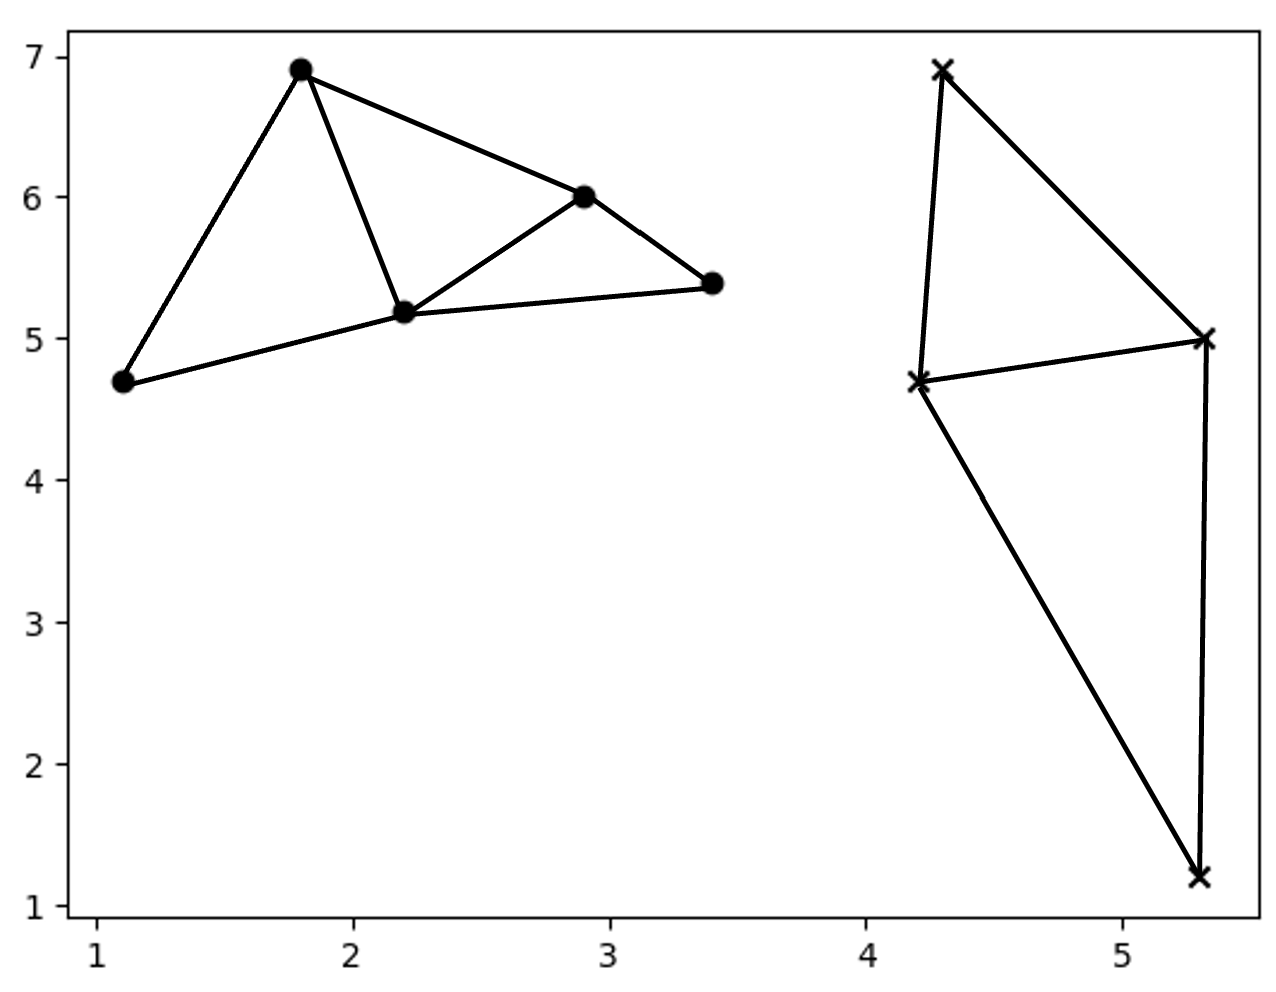
\includegraphics[width=6cm]{Note Files/ConvexHull1.png}
    \caption[name = figure]{Separable}
    \end{minipage}
    \begin{minipage}[t]{0.48\textwidth}
    \centering
    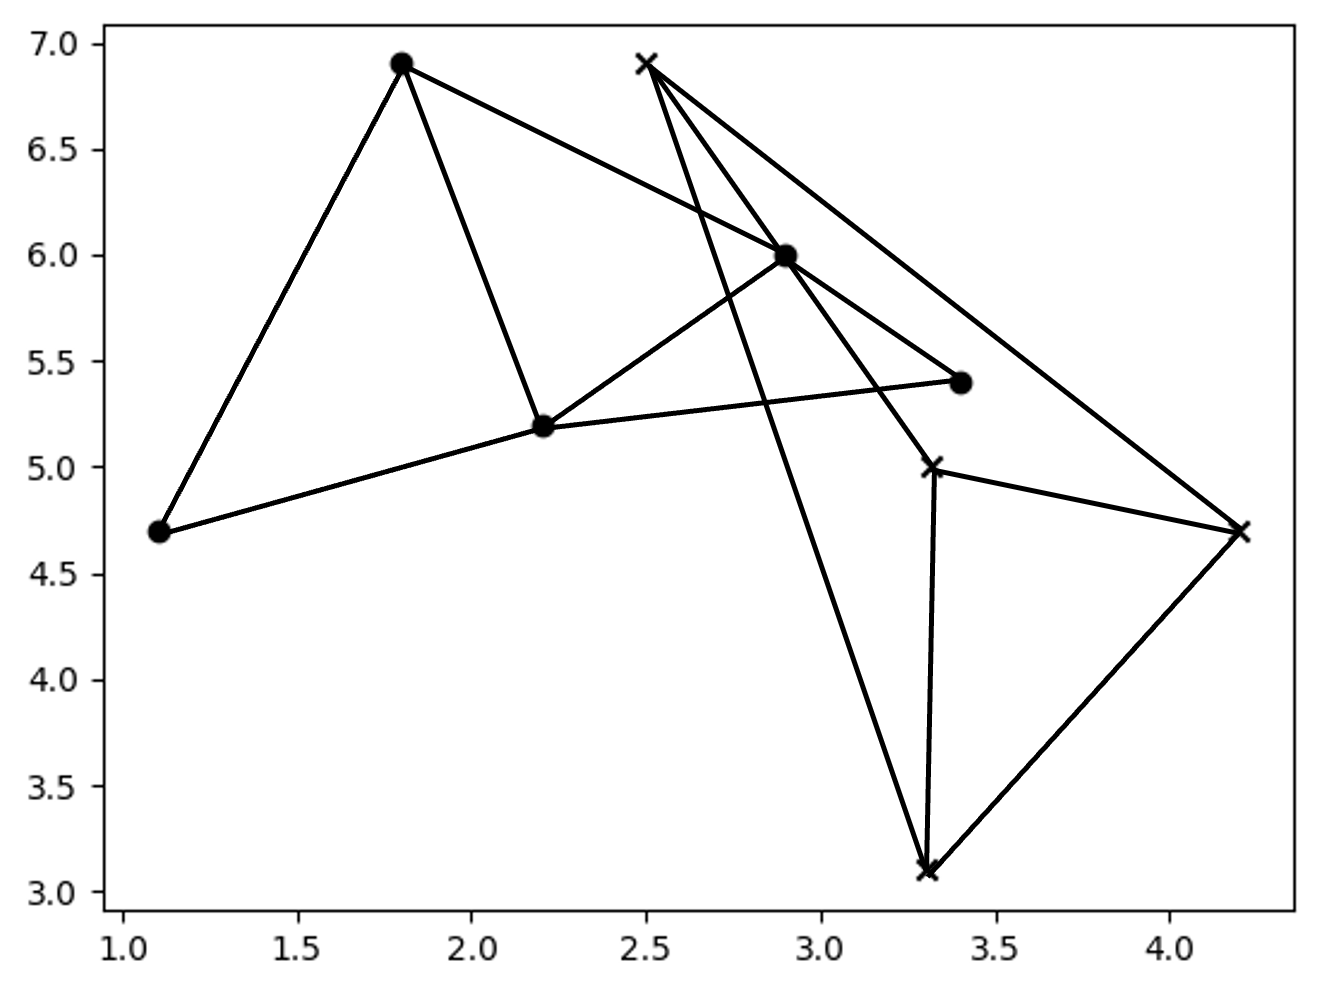
\includegraphics[width=6cm]{Note Files/ConvexHull.png}
    \caption{Not Separable}
    \end{minipage}
    \end{figure}
To cancel out the effect of some specific data points, we introduce \textbf{slack variable} $\xi_i$ for each data pair $(\bm{x}_i, y_i)$, and define the \textbf{soft geometric margin} as
\begin{equation}
    \gamma = \frac{y_i(\bm{w}^T \bm{x}_i + b) + \xi_i}{||\bm{w}||}
\end{equation}
Then for each slack variable, the target function gains a relevant penalty $C\xi_i$. Then the equivalent problem is
\begin{gather}
    \arg \max_{\bm{\alpha}} \min_{\bm{w},\bm{\xi},b} \frac{1}{2}||\bm{w}||^2 + C\sum_{i=1}^N \xi_i \notag \\ \text{s.t.}~y_i(\bm{w}^T \bm{x}_i + b) \geq 1 - \xi_i,~~\xi_i \geq 0,~
\end{gather}
Lagrange function with double multipliers $(\bm{\alpha}, \bm{\mu})$ is
\begin{equation}
    L(\bm{\alpha}, \bm{w}, \bm{\xi}, b) = \frac{1}{2}||\bm{w}||^2 + C\sum_{i=1}^N \xi_i - \sum_{i=1}^N \alpha_i \left( y_i(\bm{w}^T\bm{x}_i + b) - 1 + \xi_i \right) - \sum_{i=1}^N \mu_i \xi_i
\end{equation}
with the dual problem
\begin{equation}
    \arg \max_{\bm{\alpha}} \min_{\bm{w},\bm{\xi},b}L(\bm{\alpha}, \bm{w}, \bm{\xi}, b)~~~\text{s.t.}~\alpha_i \geq0,~\mu_i \geq 0
\end{equation}
then
\begin{equation}
    \frac{\partial}{\partial \bm{w}} L = \frac{\partial}{\partial \bm{x}_i} L = \frac{\partial}{\partial b} L = 0 \longrightarrow
\left\{ \begin{aligned}
    &\bm{w} = \sum_{i=1}^N \alpha_i y_i \bm{x}_i \\
    &\sum_{i=1}^N \alpha_i y_i = 0\\
    &C - \alpha_i - \mu_i = 0,~~\alpha_i \geq 0,~\mu_i \geq 0 \rightarrow 0 \leq \alpha_i \leq C
\end{aligned}
\right.
\end{equation}
Likewise, we obtain a new \textbf{quadratic programming} target
\begin{gather}
    \arg \min_{\bm{\alpha}} \frac{1}{2}\sum_{i=1}^N \sum_{j=1}^N \alpha_i \alpha_j y_i y_j \langle \bm{x}_i, \bm{x}_j \rangle - \sum_{i=1}^N \alpha_i  \notag \\ \text{s.t.}~\sum_{i=1}^N \alpha_i y_i = 0,~0 \leq \alpha_i \leq C
\end{gather}
\subsection{Hinge Loss Function}
We can give an equivalent description of the original optimizing problem. The minimizing part gives
\begin{equation}
    \arg \min_{\bm{w},\bm{\xi},b} \frac{1}{2}||\bm{w}||^2 + C\sum_{i=1}^N \xi_i,~~\text{s.t.}~~y_i(\bm{w}^T \bm{x}_i + b) \geq 1 - \xi_i,~\xi_i \geq 0
\end{equation}
If we take 
\begin{equation}
    \left[1 - y_i(\bm{w}^T \bm{x}_i + b)\right]_+ = \xi_i~~~\left( f(x)_+ = \left\{ \begin{aligned} & f(x) &f(x) > 0 \\ &0 &x \leq 0 \end{aligned} \right. \right)
\end{equation}
Then if $1 - y_i(\bm{w}^T \bm{x}_i + b) > 0$, then $y_i(\bm{w}^T \bm{x}_i + b) = 1 - \xi_i$. If $1 - y_i(\bm{w}^T \bm{x}_i + b) \leq 0$, then $\xi_i = 0$. It meets the condition that $y_i(\bm{w}^T \bm{x}_i + b) \geq 1 - \xi_i $. Hence, the minimization can be rewritten as
\begin{equation}
    \arg \min_{\bm{w}, \bm{\xi}, b} \frac{1}{2C} ||\bm{w}||^2 + \sum_{i=1}^N \xi_i \stackrel{\lambda = 1/2C}{\longrightarrow} \arg \min_{\bm{w}, b} \lambda ||\bm{w}||^2 + \sum_{i=1}^N \left[1 - y_i(\bm{w}^T \bm{x}_i + b)\right]_+
\end{equation}
Then loss function $\left[1 - y_i(\bm{w}^T \bm{x}_i + b)\right]_+$ on the RHS is defined as the \textbf{hinge loss function}, which requires a higher standard for sample studying.
\subsection{Kernel Trick for Non-linear SVM}
The linear separable and linear inseparable sample can be split using a hyperplane. Whereas non-linear samples require a hypersurface for partition. 
\subsubsection{Kernel Function}
Assume input space is $\mathcal{X}$ and characteristic space $\mathcal{H}$, there exists a mapping $\phi(x)$, where
\begin{equation}
    \phi(x): \mathcal{X} \mapsto \mathcal{H}
\end{equation}
such that $\forall x, y \in \mathcal{X}$,
\begin{equation}
    K(x,y) = \left\langle \phi(x),\phi(y) \right\rangle
\end{equation}
then $K(x, y)$ is the kernel function, and $\phi(x)$ is the mapping function. For a given kernel $K(x, y)$, the selection for characteristic space and mapping function is not unique. \par
In non-linear SVM, we take the place of inner function in the optimization by the kernel function, i.e.
\begin{gather}
    \arg \min_{\bm{\alpha}} \frac{1}{2}\sum_{i=1}^N \sum_{j=1}^N \alpha_i \alpha_j y_i y_j K(\bm{x}_i,\bm{x}_j) - \sum_{i=1}^N \alpha_i  \notag \\ \text{s.t.}~\sum_{i=1}^N \alpha_i y_i = 0,~0 \leq \alpha_i \leq C
\end{gather}
\subsubsection{Positive Definite Kernel Function}
The following will give the necessary and sufficient condition for $K(x, y)$ to be \textbf{positive definite kernel}. We first consider mapping function
\begin{equation}
    \phi: x \mapsto K(\bdot, x)
\end{equation}
Then $\forall x_i \in \mathcal{X},\alpha_i \in \mathbb{R}$, define linear mapping
\begin{equation}
    f(\bdot) = \sum_{i=1}^N \alpha_i K(\bdot, x_i)
\end{equation} 
the space $\mathcal{S}$ is determined by mapping $\phi$. Define operation $\langle f, g, \rangle$ in space $\mathcal{S}$ for $f, g$, where
\begin{gather}
    f(\bdot) = \sum_{i=1}^N \alpha_i K(\bdot, x_i),~~
    g(\bdot) = \sum_{j=1}^N \beta_j K(\bdot, y_j) \\
    \langle f, g \rangle = \sum_{i=1}^N\sum_{j=1}^N \alpha_i \beta_j K(x_i, y_j)
\end{gather}
\rule[-5pt]{\linewidth}{0.07em}
\noindent \textbf{Lemma 1} The operation is a inner product of $\mathcal{S}$.
\begin{gather}
    \sum_{i=1}^N\sum_{j=1}^N C\alpha_i \beta_j K(x_i, y_j) = C\sum_{i=1}^N\sum_{j=1}^N \alpha_i \beta_j K(x_i, y_j) \longrightarrow \la Cf, g \ra = C\la f, g \ra \\
    \la f, g \ra = \la g, f \ra~~(\text{trivial}) \\
    \sum_{i=1}^N\sum_{j=1}^N \left( (\alpha_i + \beta_i) \gamma_j K(y_i, z_j) \right) = \sum_{i=1}^N\sum_{j=1}^N  \alpha_i \gamma_j K(x_i, z_j) + \sum_{i=1}^N \sum_{j=1}^N \beta_i \gamma_j K(y_i, z_j) \notag\\ \rightarrow \la f+g, h \ra = \la f, h \ra + \la g, h \ra \\
    \la f, f \ra = \sum_{i=1}^N \sum_{j=1}^N \alpha_i \alpha_j K(x_i, x_j) = \bm{\alpha}^TG_{\bm{x}}\bm{\alpha} \geq 0 
\end{gather}
The following will give the proof that $\la f, f \ra = 0$ if and only if $f(\bdot) = 0$. Necessity is trivial. It is evident that $\mathcal{S}$ is a closure, then $\forall f, g \in \mathcal{S}, \lambda \in \mathbb{R}$, $f + \lambda g \in \mathcal{S}$. Then
\begin{gather}
    \la f + \lambda g, f + \lambda g \ra = \la f, f \ra + 2\lambda \la f, g \ra + \lambda^2 \la g, g \ra \geq 0 \notag \\
    \Delta = 4\left(|\la f, f \ra |^2 - \la f, f \ra \la g, g \ra \right) \leq 0 \rightarrow |\la f, f \ra |^2 - \la f, f \ra \la g, g \ra \leq 0
\end{gather}
then
\begin{equation}
    \forall x \in \mathcal{X}, \la K(\bdot, x), f(\bdot)\ra = \sum_{i=1}^N \alpha_i \la K(\bdot, x), K(\bdot, x_i) \ra= f(x) 
\end{equation}
with the inequality above,
\begin{equation}
    |\left\la K(\bdot, x), f(\bdot)\right\ra|^2 \leq \la K(\bdot, x), K(\bdot, x) \ra \la f(\bdot), f(\bdot) \ra
\end{equation}
Where
\begin{equation}
    \la K(\bdot, x), K(\bdot, x) \ra = K(x, x)
\end{equation}
then
\begin{equation}
    |f(x)|^2 \leq K(x, x) \la f(\bdot), f(\bdot) \ra
\end{equation}
then if $\la f,f \ra = 0$, $f(x) = 0$ must holds for all $x$
. We can conclude that operation $\la f, g \ra $ on $f, g$ is a well-defined inner product. \par \noindent
\rule[-0em]{\linewidth}{0.07em}
Define norm $||f||$ for all $f \in \mathcal{S}$ as follows
\begin{equation}
    ||f|| = \sqrt{\la f, f \ra}
\end{equation}
then $\mathcal{S}$ is completed as an Hilbert space $\mathcal{H}$, named \textbf{reproducing kernel Hilbert space}, for kernel $K$ has reproducibility, i.e. $\la K(\bdot, x), f \ra = f(x)$, $\la K(\bdot, x), K(x, \bdot) \ra = K(x, x)$. We can conclude that
\begin{equation}
    \boxed{\text{Any kernel function $K$ implicitly defines a reproducing kernel Hilbert space}} \notag
\end{equation}
\rule[0em]{\linewidth}{0.07em}
\textbf{Lemma 2} Kernel $K$ is a positive definite kernel if and only if the Gram matrix of $K$ is half positive definite. \par Necessity: If $G_K$ is half positive definite for arbitrary $\bm{x}$, then as shown above, $K$ determines a RKHS, that is, $\la K(\bdot, x), f \ra = f(x)$, $\la K(\bdot, x), K(x, \bdot) \ra = K(x, x)$ holds. a mapping $\phi: x \mapsto K(\bdot, x) \leftrightarrow \mathcal{H}$ can be built up by defining
\begin{equation}
    K(x, y) = \la \phi(x), \phi(y) \ra
\end{equation} \par
Sufficiency: If $K$ is a positive definite kernel, then $K(x, y) = \la \phi(x), \phi(y) \ra$. Hence $\forall \bm{\alpha} \in \mathbb{R}^N$,
\begin{equation}
    \bm{\alpha}^T G_{K} \bm{\alpha} = \sum_{i=1}^N \alpha_i \sum_{j=1}^N \alpha_j \la \phi(x_i), \phi(y_i) \ra = \left\la \sum_{i=1}^N \alpha_i \phi(x_i) , \sum_{j=1}^N \alpha_j \phi(y_j) \right\ra \geq 0
\end{equation}
then $G_K$ is half positive definite. QED
\subsubsection{Normally-used Kernel Function}
\noindent \textbf{Linear/Polynomial Kernel} 
\begin{equation}
    K(x, y) = \la x, y \ra^d
\end{equation}
\textbf{Gaussian/Laplacian Kernel}
\begin{equation}
    K(x, y) = -\frac{||x - y||^2}{2\sigma^2} \bigg/ -\frac{||x-y||}{\sigma}
\end{equation}
\textbf{Sigmoid Kernel}
\begin{equation}
    K(x, y) = \tanh \left( \beta \la x, y \ra + \theta\right)
\end{equation}
\subsection{Coordinate Descent}
One basic algorithm to search for the lagrange multiplier matrix is the coordinate descent. The following gives the iteration
\begin{algorithm}[H]
    \caption{coordinateDescent($\bm{\alpha}$)}
    \label{coorDes}
    \begin{algorithmic}
        \WHILE{not converge}
        \FOR{$i = 0$ \TO $N$}
        \STATE{$\alpha_i := \arg \min_{\hat \alpha_i} W(\alpha_1, \alpha_2, \dots, \alpha_{i-1}, \hat \alpha_{i}, \alpha_{i+1}, \dots, \alpha_N)$ s.t. $\hat \alpha_i = -\sum_{j\neq i} \alpha_j$}
        \ENDFOR
        \ENDWHILE
    \end{algorithmic}
\end{algorithm}
The inner loop search the minima of $W$ with one variable $\alpha_i$ at one time.
\subsection{Sequential Minimization Optimization}
If we deal with two variables $\alpha_i, \alpha_j$ chosen at random on optimizing the convex optimization (due to the constraint condition). Apart from the pivot $(\alpha_i, \alpha_j)$ we have other variables fixed. Then $(\alpha_i, \alpha_j)$ constructs a partition for the original quadratic programming problem.
Then the constraint condition is expanded to
\begin{gather}
    \arg \min_{\alpha_i, \alpha_j} \frac{1}{2} \alpha_i^2 K(x_i, x_i) + \frac{1}{2}\alpha_j^2 K(x_j, x_j) + \alpha_i\alpha_j y_i y_j K(x_i, x_j) - (\alpha_i + \alpha_j) \notag \\ + \alpha_i y_i \sum_{k\neq i} \alpha_k y_k K(x_i, x_k) + \alpha_j y_j \sum_{k\neq j}
    \alpha_k y_k K(x_j, x_k) - \sum_{k\neq i, j} \alpha_k \\
    \text{s.t.}~~\alpha_iy_i + \alpha_jy_j = -\sum_{k \neq i,j}^N \alpha_k y_k =   \zeta,~0 \leq \alpha_i, \alpha_j \leq C
\end{gather}
Then constraint condition is shown as
\begin{equation}
    \left\{ \begin{aligned}
        &\alpha_i + \alpha_j = \zeta / y_i &y_i = y_j \\
        &\alpha_i - \alpha_j = \zeta / y_i &y_i \neq y_j
    \end{aligned} \right.
\end{equation}
And in the optimizing iteration the equality
\begin{equation}
    \alpha_i^{\new}y_i + \alpha_j^{\new}y_j = \zeta = \alpha_i^{\old}y_i + \alpha_j^{\old}y_j
\end{equation}
then the constraint condition for $\alpha_j^{\new}$ is
\begin{equation}
    L \leq \alpha_j^{\new} \leq H,~~(L, H) = \left\{ \begin{aligned}
        &\left( \max(0, \alpha_j^{\old} - \alpha_i^{\old}), \min(C, C+\alpha_j^{\old} - \alpha_i^{\old}) \right) &y_i = y_j \\
        &\left( \max(0, \alpha_j^{\old} + \alpha_i^{\old} - C), \min(C, \alpha_j^{\old} + \alpha_i^{\old})\right) &y_i \neq y_j
    \end{aligned} \right.
\end{equation}
With $\alpha_iy_i = \zeta - \alpha_jy_j \rightarrow \alpha_i = y_i(\zeta - \alpha_jy_j)$, target expands to
\begin{gather}
    \arg \min_{\alpha_j} W(\alpha_j) \notag \\= \frac{1}{2}\alpha_i^2K(x_i, x_j) + \frac{1}{2}\alpha_j^2K(x_j, x_j) + \alpha_i\alpha_jy_iy_jK(x_i, x_j)-(\alpha_i+\alpha_j) + \alpha_iy_iv_i+\alpha_jy_jv_j \\
    \text{where}~~v_i = \sum_{k\neq i} \alpha_k y_k K(x_i, x_k)
\end{gather}
then
\begin{equation}
    \frac{\partial}{\partial \alpha_j}W(\alpha_j) = 0 \rightarrow \alpha_j = y_j \frac{y_j - y_i + \zeta(K(x_i, x_i) - K(x_i, x_j))+v_i - v_j}{K(x_i,x_i) + K(x_j, x_j) - 2K(x_i, x_j)}
\end{equation}
\end{document}